\tikzstyle{startstop} = [rectangle, rounded corners, minimum width=3cm, minimum height=1cm,text centered, draw=black, fill=gray!20]
\tikzstyle{process} = [rectangle, minimum width=3cm, minimum height=1cm, text centered, draw=black, fill=blue!10]
\tikzstyle{arrow} = [thick,->,>=stealth]

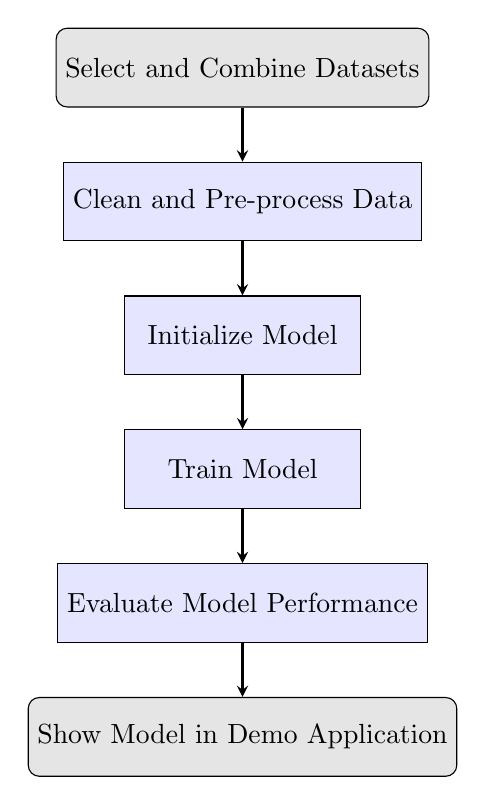
\begin{tikzpicture}[node distance=1.7cm]

\node (start) [startstop] {Select and Combine Datasets};
\node (clean) [process, below of=start] {Clean and Pre-process Data};
\node (features) [process, below of=clean] {Initialize Model};
\node (train) [process, below of=features] {Train Model};
\node (evaluate) [process, below of=train] {Evaluate Model Performance};
\node (demo) [startstop, below of=evaluate] {Show Model in Demo Application};

\draw [arrow] (start) -- (clean);
\draw [arrow] (clean) -- (features);
\draw [arrow] (features) -- (train);
\draw [arrow] (train) -- (evaluate);
\draw [arrow] (evaluate) -- (demo);

\end{tikzpicture}
